% Share of eligible applicants choosing the GF (pooled 2016-2020) against reviewer disagreement
% (1 - Gwet's AC, 0-5 grade, power-1/4 weights, IF 2014-2018 reviewer scores), by MSCA panel; all eight panels.
% GENERATED BY msca_figures.py - edit that file, not this one.
% CHE: 1-AC 0.488 (SE 0.0046), GF 318 of 5617 = 5.66%; ECO: 1-AC 0.550 (SE 0.0108), GF 97 of 967 = 10.03%; ENG: 1-AC 0.543 (SE 0.0047), GF 511 of 5233 = 9.76%; ENV: 1-AC 0.525 (SE 0.0044), GF 655 of 5297 = 12.37%; LIF: 1-AC 0.501 (SE 0.0031), GF 867 of 9815 = 8.83%; MAT: 1-AC 0.508 (SE 0.0110), GF 66 of 961 = 6.87%; PHY: 1-AC 0.442 (SE 0.0049), GF 393 of 4661 = 8.43%; SOC: 1-AC 0.595 (SE 0.0035), GF 1412 of 9861 = 14.32%
% fits (share on disagreement): all: slope 44.2 pp per unit, R2 0.52, p 0.043; nophy: slope 70.0 pp per unit, R2 0.72, p 0.016; nosoc: slope 28.9 pp per unit, R2 0.23, p 0.271
\definecolor{msca1}{HTML}{2A78D6}
\begin{figure}[htbp]
\centering
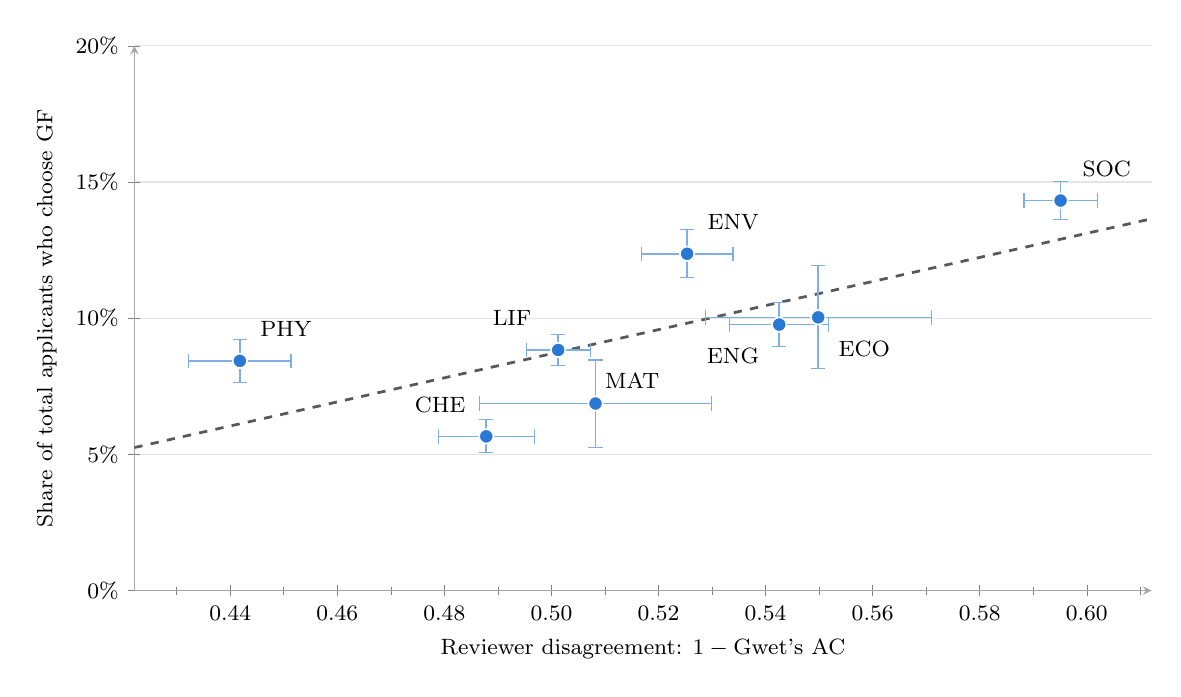
\begin{tikzpicture}
\begin{axis}[
  width=14.5cm, height=8.5cm,
  xmin=0.4221, xmax=0.6121, ymin=0, ymax=20,
  xtick distance=0.02, minor x tick num=1,
  xticklabel style={/pgf/number format/.cd, fixed, fixed zerofill, precision=2},
  ytick distance=5, yticklabel={\pgfmathprintnumber{\tick}\%},
  axis x line=bottom, axis y line=left, axis line style={gray!70},
  ymajorgrids, grid style={gray!20},
  tick label style={font=\footnotesize}, label style={font=\footnotesize},
  xlabel={Reviewer disagreement: $1-{}$Gwet's AC},
  ylabel={Share of total applicants who choose GF},
  clip=false,
]
\addplot[gray!70!black, line width=1pt, dashed, domain=0.4221:0.6121, samples=2] {-13.40933+44.20834*x};
\addplot[only marks, mark=*, mark size=2.6pt, color=msca1, forget plot,
  mark options={fill=msca1, draw=white, line width=0.6pt},
  error bars/.cd, x dir=both, x explicit, y dir=both, y explicit,
  error bar style={color=msca1!60, line width=0.6pt}]
  table[row sep=\\, x=d, y=s, x error=dx, y error=ds]
  {d s dx ds \\ 0.48782 5.6614 0.00895 0.6044 \\ 0.54983 10.0310 0.02108 1.8935 \\ 0.54254 9.7650 0.00922 0.8043 \\ 0.52534 12.3655 0.00857 0.8865 \\ 0.50126 8.8334 0.00600 0.5614 \\ 0.50823 6.8678 0.02161 1.5990 \\ 0.44180 8.4317 0.00956 0.7977 \\ 0.59510 14.3190 0.00684 0.6913 \\};
\node[font=\footnotesize, anchor=center] at (axis cs:0.47920,6.8208) {CHE};
\node[font=\footnotesize, anchor=center] at (axis cs:0.55845,8.8716) {ECO};
\node[font=\footnotesize, anchor=center] at (axis cs:0.53392,8.6055) {ENG};
\node[font=\footnotesize, anchor=center] at (axis cs:0.53396,13.5249) {ENV};
\node[font=\footnotesize, anchor=center] at (axis cs:0.49264,9.9928) {LIF};
\node[font=\footnotesize, anchor=center] at (axis cs:0.51508,7.6794) {MAT};
\node[font=\footnotesize, anchor=center] at (axis cs:0.45042,9.5911) {PHY};
\node[font=\footnotesize, anchor=center] at (axis cs:0.60372,15.4785) {SOC};
\end{axis}
\end{tikzpicture}
\caption{\footnotesize Share of eligible applicants who applied to the Global rather than the European
Fellowship, pooled over 2016--2020, against reviewer disagreement, by MSCA panel. Disagreement is one minus
Gwet's AC, computed from the three reviewer scores of each submission in 2014--2018,
grouped into the six grades of the 0--5 scale used to evaluate application proposals in the GF/EF program. Bars are 95 percent
confidence intervals.
CHE: chemistry; ECO: economics; ENG: information science and engineering; ENV: environment and geosciences;
LIF: life sciences; MAT: mathematics; PHY: physics; SOC: social sciences and humanities.}
\label{fig:msca_noise_share}
\end{figure}
